\section{Aplicaciones}
\label{aplicaciones}

Los m\'aseres tienen diferentes aplicaciones, principalmente como osciladores (referencias de frecuencia en relojes at\'omicos) y amplificadores de bajo nivel de ruido. En esta secci\'on se describir\'an brevemente estas aplicaciones y otras.

\subsection{Oscilador}

A pesar de la denominaci\'on de amplificadores que tambi\'en se les da, el uso m\'as corriente que se hace de los m\'aseres es como osciladores, sobre todo cuando trabajan a frecuencias elevadas (longitudes de onda submilim\'etricas) para las que, por otra parte, constituyen el \'unico procedimiento pr\'actico de obtener radiaci\'on monocrom\'atica de gran pureza y altas energ\'ias: del orden de GigaVatios (109 GW) en impulsos y de varios centenares de Vatios en onda continua \cite{spiritusTemporis}. 

\subsection{Relojes at\'omicos}
Los m\'asers oscilan a la frecuencia de resonancia del \'atomo o mol\'ecula que los produce con un ancho de banda muy estrecho. Esto hace que sean buenas referencias de frecuencia de alta precici\'on, por lo que sirven, por ejemplo, como relojes at\'omicos. Los m\'aseres de amon\'iaco e hidr\'ogeno se han considerado como patrones de frecuencia y se han utilizado como relojes en experimentos de comprobaci\'on de la relatividad especial.

Un reloj at\'omico es un tipo de reloj que usa una frecuencia de resonancia at\'omica est\'andar como contador. Los primeros relojes at\'omicos eran m\'aseres con cierto equipamiento adicional. Hoy en d\'ia, aunque los m\'aseres se siguen usando en muchos relojes at\'omicos, los est\'andares de frecuencia m\'as avanzados se basan en procesos f\'isicos m\'as avanzados que involucran \'atomos fr\'ios y las fuentes at\'omicas.

El primer reloj at\'omico fue construido en 1949 en la Ofinina Nacional de Normalizaci\'on de los Estados Unidos bas\'andose en las ideas sobre un fen\'omeno extremadamente regular: la resonancia magn\'etica molecular y at\'omica. Sin embargo, la precisi\'on conseguida por el amon\'iaco (mol\'ecula utilizada por este primer prototipo) no era muy superior a los est\'andares de la \'epoca basados en osciladores de cuarzo. En 1955 Louis Essen construy\'o el primer reloj at\'omico realmente preciso en el Reino Unido, bas\'andose en la transici\'on del \'atomo Cesio-133 (que no es un m\'aser). Esto llev\'o a la definici\'on del segundo basada en el tiempo at\'omico. M\'as adelante se crearon m\'aseres de hidr\'ogeno, con una precisi\'on mayor.

La Figura \ref{fig:atomic_clock_gps} muestra un reloj at\'omico hecho a partir de un m\'aser de hidr\'ogeno situado en Canad\'a y perteneciente a la red de posicionamiento global GPS.

\begin{figure}[ht!!]
 \centering
 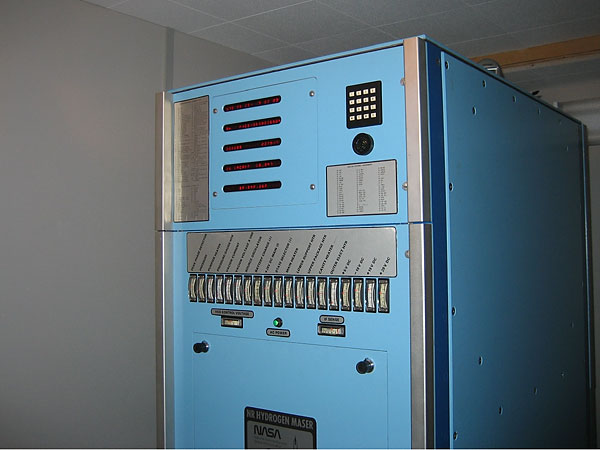
\includegraphics[width=0.5\textwidth]{./Utils/atomic_clock_gps.jpg}
 % atomic_clock_gps.jpg: 600x450 pixel, 100dpi, 15.24x11.43 cm, bb=0 0 432 324
 \caption{Reloj atómico del sistema GPS}
 \label{fig:atomic_clock_gps}
\end{figure}


Dispositivos como los relojes at\'omicos que producen este tipo de mediciones resultan esenciales para la vida moderna. S\'olo gracias a esta exactitud se pueden realizar conexiones v\'ia sat\'elite y funcionan los dispositivos GPS, entre otras cosas. El GPS, de hecho, se basa en dos docenas de satélites, cada uno con cuatro relojes atómicos. Por medio de la triangulación de las señales de tiempo que se emiten desde la órbita, los receptores en el planeta brindan a los usuarios su localización con un alto grado de exactitud.

\subsection{Amplificador de bajo nivel de ruido}

Otra aplicaci\'on de los m\'aseres es la de amplificadores de bajo nivel de ruido, especialmente en radiotelescopios.

Los amplificadores m\'aser tienen un nivel de ruido interno incre\'iblemente bajo, lo que hace que sean extremadamente sensibles. Estas caracter\'isticas hacen que estos dispositivos sean particularmente \'utiles para recepci\'on y detecci\'on de se\~nales muy d\'ebiles en radioastronom\'ia, radiometr\'ia de microondas y aplicaciones similares.

Sin embargo, el uso de amplificadores m\'aser supone un coste elevado, por lo que se utilizan \'unicamente en aquellos casos en que el bajo nivel de ruido requerido justifique el alto coste y la resoluci\'on de los problemas tecnol\'ogicos que surgen, principalmente al tener que utilizar bajas temperaturas. Por ejemplo, se utilizan para detecci\'on de radiaci\'on espacial y comunicaciones con sat\'elites, adem\'as de las aplicaciones mencionadas antes.

La Figura \ref{fig:amplificador_cavidad} muestra un amplificador m\'aser del tipo \textit{cavidad de transmisi\'on}. En amplificadores m\'aser con esta estructura es normal colocar aisladores de ferrita en las gu\'ias de entrada y de salida para proteger al m\'aser de reflexiones que se puedieran producir en la carga. 

\begin{figure}[ht!!]
 \centering
 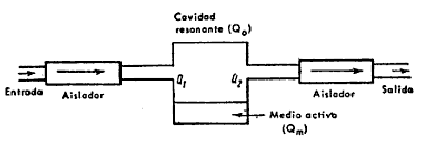
\includegraphics[width=0.7\textwidth]{./Utils/amplificador_transmision.png}
 % atomic_clock_gps.jpg: 600x450 pixel, 100dpi, 15.24x11.43 cm, bb=0 0 432 324
 \caption{Amplificador m\'aser de cavidad de transmisi\'on}
 \label{fig:amplificador_cavidad}
\end{figure}

Como ejemplo de aplicaci\'on pr\'actica, se ha utilizado un amplificador m\'aser en experimentos que detectaban la radiaci\'on c\'osmica generada por el Big Bang que cre\'o el universo.

\subsection{Otras aplicaciones}

Los m\'aseres se utilizan habitualmente como amplificadores, osciladores o relojes at\'omicos. Sin embargo, \'esas no son todas las funciones que pueden cumplir. Por ejemplo, se utilizan en laboratorios para hacer experimentos de mec\'anica cuantica e intentar descubrir nuevas caracter\'isticas de la materia y obtener m\'as informaci\'on sobre los movimientos de los \'atomos. 

Adem\'as, actualmente se est\'an investigando otras posibles aplicaciones de estos dispositivos. El ej\'ercito de los Estados Unidos, por ejemplo, est\'a haciendo pruebas con los m\'aseres como armas disuasorias. Los m\'aseres emiten frecuencias de microondas y, si se apunta con ellos a personas, producen un calentamiento en el agua de la piel. Aunque en principio esto no es peligroso si no se radia durante mucho tiempo a la misma zona, produce una sensaci\'on inc\'omoda en los afectados.

\newpage
\section{Ejemplo de aplicaci\'on pr\'actica}
En esta secci\'on se describir\'a una aplicaci\'on pr\'actica del dispositivo m\'aser: el m\'aser MHM 2010 \cite{MHM2010}, que es un reloj at\'omico de hidr\'ogeno.

\subsection{Caracter\'isticas}
El MHM 2010 es el único maser activo de hidrógeno disponible en el mercado con cavidad independiente. Esto le permite mantener una estabilidad buena durante un largo periodo de tiempo, atributo que únicamente se atribuía a los maseres de cesio.


\begin{figure}[htb!!]
 \centering
 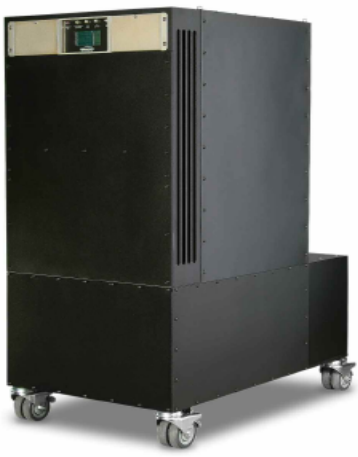
\includegraphics[width=0.3\textwidth]{./Utils/maser_MHM.png}
 % varianzaAllen.png: 607x475 pixel, 101dpi, 15.27x11.95 cm, bb=0 0 433 339
 \label{fig:imagen_maser}
 \caption{M\'aser MHM 2010}
\end{figure}

Este m\'aser puede emitir a tres frecuencias diferentes, teniendo las tres la misma amplitud. En la Tabla \ref{table:amplitud} se muestran las medidas de amplitud tomadas a diferentes frecuencias para una carga de 50 \ohm.

\begin{table}[htb]
\begin{center}
\begin{tabular}[t]{|l|l|}
\hline \hline
\rowcolor[RGB]{244, 184, 184} \textbf{Frecuencia (MHz)} & \textbf{Amplitud (dBm)}\\
\hline \hline
5 & 13\\
\hline
10 & 13\\
\hline
100 & 13\\
\hline\hline
\end{tabular}
\end{center}
\caption{Amplitud del m\'aser a diferentes frecuencias}
\label{table:amplitud}
\end{table}

A medida que aumentamos la frecuencia el ruido de fase va disminuyendo, tal como se muestra en la Tabla \ref{table:ruido_fase}

\begin{table}[htb]
\begin{center}
\begin{tabular}[t]{|l|l|l|}
\hline \hline
\rowcolor[RGB]{244, 184, 184} \textbf{Frecuencia} & \textbf{M\'aser a 5 MHz} & \textbf{M\'aser a 10 MHz}\\
\hline \hline
1 Hz & $\leq$ -112 dBc & $\leq$ -106 dBc\\
\hline
10 Hz & $\leq$ -130 dBc & $\leq$ -124 dBc\\
\hline 
100 Hz& $\leq$ -148 dBc & $\leq$ -142 dBc\\
\hline 
1 KHz& $\leq$ -155 dBc & $\leq$ -149 dBc\\
\hline 
10 KHz& $\leq$ -155 dBc & $\leq$ -149 dBc\\
\hline
100 KHz& $\leq$ -155 dBc & $\leq$ -149 dBc\\
\hline\hline
\end{tabular} 
\end{center}
\caption{Ruido de fase del m\'aser en funci\'on de la frecuencia}
\label{table:ruido_fase}
\end{table}


Como se ha dicho al principio de este punto, este m\'aser presenta una buena estabilidad, incluso tras haber transcurrido un largo tiempo. En la Figura \ref{fig:varianza_allan} se muestra la caracter\'istica de este oscilador (su varianza de Allan\footnote{Para caracterizar la estabilidad en frecuencia de los osciladores se utiliza la varianza de Allan, porque no presenta ambigüedades ni inconsistencias en su caracterizaci\'on. }), mostrando el tiempo en el eje \textit{x} y la desviaci\'on producida en el eje \textit{y}.

\begin{figure}
 \centering
 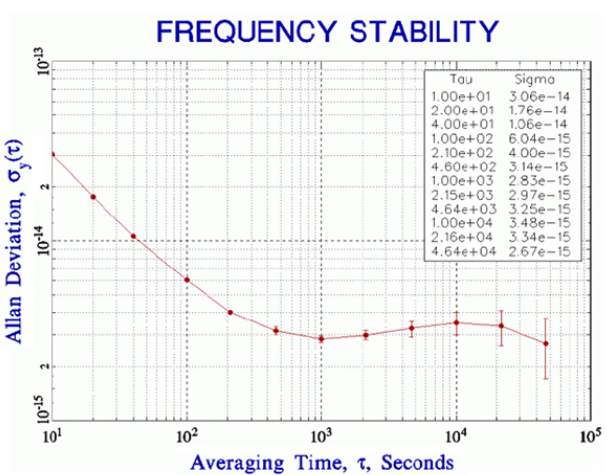
\includegraphics[width=0.8\textwidth]{./Utils/varianzaAllen.png}
 % varianzaAllen.png: 607x475 pixel, 101dpi, 15.27x11.95 cm, bb=0 0 433 339
 \caption{Estabilidad en frecuencia del oscilador}
 \label{fig:varianza_allan}
\end{figure}

Este m\'aser funciona con un voltaje comprendido entre 85 y 264 VAC, de 47 a 63 Hz de frecuencia. Si trabaja con continua requiere de 22 a 28 voltios con una intensidad típica de 3.1 amperios. En este caso tiene un tiempo de trabajo de 8 horas.

\subsection{Funcionamiento}

A continuaci\'on se explica el funcionamiento de este m\'aser de hidr\'ogeno a partir de su diagrama de bloques (ver Figura  \ref{fig:maser_desglosado}). Para simplificar el diagrama se han destacado \'unicamente las partes propias del m\'aser, dejando de lado las de control. 

\begin{figure}[hb!!!]
 \centering
 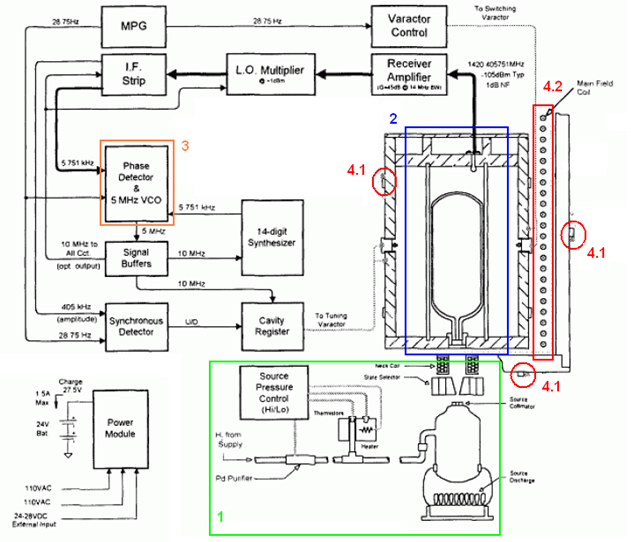
\includegraphics[width=\textwidth]{./Utils/maser_desglosado.png}
 % varianzaAllen.png: 607x475 pixel, 101dpi, 15.27x11.95 cm, bb=0 0 433 339
 \caption{Esquema del funcionamiento del maser}
 \label{fig:maser_desglosado}
\end{figure}

1. Fuente de hidrógeno y puertas magnéticas que permiten el paso de ciertas moléculas.

2. Cavidad de resonancia.

3. PLL y VCO para generar la señal de salida.

4. Control de temperatura. Para ello se realiza mediante termistores (4.1), que son resistencias cuyo valor varía con la temperatura, y un escudo térmico (4.2).


Para explicar mejor su funcionamiento se prestará mayor atención a la Figura \ref{fig:esquema_maser}, ya que visualiza esquemáticamente las partes involucradas.

\begin{figure}[hb!!]
 \centering
 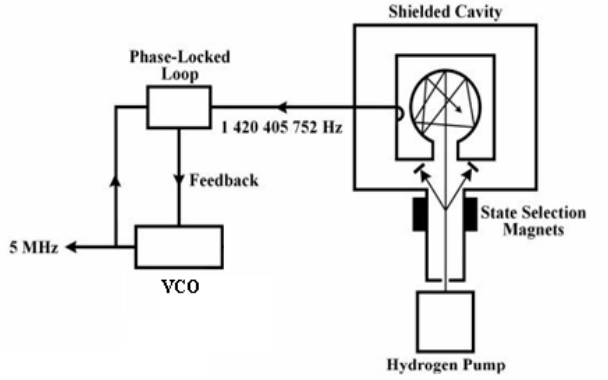
\includegraphics[width=0.7\textwidth]{./Utils/maser_esquema.png}
 % varianzaAllen.png: 607x475 pixel, 101dpi, 15.27x11.95 cm, bb=0 0 433 339
 \caption{Esquema del m\'aser}
 \label{fig:esquema_maser}
\end{figure}

Como se ha explicado en el punto \ref{tipo:hidrogeno}. \nameref{tipo:hidrogeno}, los m\'asers de hidrogeno funcionan a la frecuencia de resonancia del átomo de hidrógeno, que es 1420 MHz. 

Un máser de hidrógeno funciona mediante el envío de gas de hidrógeno a través de una puerta magnética que sólo permite que los átomos con cierta energía pasen a través. 

Los átomos que atraviesan la puerta entran en una bombilla de almacenamiento rodeada por una cavidad resonante. Una vez dentro de la bombilla, cuando alcanzan un estado energético menor, liberan fotones a frecuencias de microondas. Estos fotones estimulan otros átomos a abandonar su nivel de energía, y ellos a su vez liberan más fotones. De esta manera, un campo de microondas autosostenible se acumula en la bombilla. La cavidad resonante que rodea la bombilla ayuda a redirigir a los fotones de nuevo al sistema para mantener la oscilación. El resultado es una señal de microondas de la frecuencia de resonancia del átomo de hidrógeno y que continuamente se emiten en función del tiempo que lleve la entrada de nuevos átomos al sistema.

Una vez generada la señal de microondas a 1420 MHz se introduce en un oscilador basado en un PLL (sistema enganchado en fase). El m\'aser dispone de un VCO que oscila a una frecuencia determinada (frecuencia de oscilación libre), que se compara con la que se ha generado en la cavidad de resonancia. Al realizar dicha comparación se generan productos de las frecuencias, que se har\'an pasar por un filtro para delimitar la frecuencia deseada.

La frecuencia de salida puede ser modificada variando la tensión de entrada del VCO, ya que al variar su tensión se var\'ia la frecuencia a la que oscila.
